% ================================================================
% CHAPTER 5: Resultate
% ================================================================


\chapter{Resultate}


Im Rahmen der vorliegenden Arbeit wurde eine Domänenanalyse zur automatischen Analyse von Kamerabildern bei der Geburt von Kälbern gemacht. Dabei wurde ein umfassendes System modelliert, welches sowohl die automatische Analyse von Kamerabildern als auch die Benachrichtigung der Stakeholder ermöglicht. Zudem erlaubt das modellierte System die Erfassung der medizinischen Daten von Kuh und Kalb. Dies ermöglicht dem Landwirten oder Tierarzt beispielsweise Zugriff auf die Krankheitsgeschichte oder den Verlauf der letzten Geburten einer Kuh. Dies unterstützt eine Beurteilung der Situation durch Fachpersonen. 

Dabei ist der Kern der Domänenanalyse die Identifikation von Geburtsmerkmalen. Im Wesentlichen hat sich ergeben, dass das System bei Erkennung von seitlichem Liegen und Anwesenheit der Wasser- oder Schleimblase eine Benachrichtigung an die Stakeholder auslösen muss. 

Der Kern des modellierten Systems wurde in Code umgesetzt. Es wurde ein flexibles und stark konfigurierbares System entwickelt, welches die automatische Analyse von Kamerabildern ermöglicht.

In den folgenden Abbildungen bedeuten grün eingefärbte Flächen, dass das System Konturen erkannt hat, diese aber nicht als Merkmal für eine Kuh in Seitenlage betrachtet. Rote Flächen bedeuten, dass das System diese Kontur als Merkmal für Seitenlage interpretiert.

In den Abbildungen \ref{fig: Korrektes Ergebnis von Analyse der stehenden Kuh} und \ref{fig: Weiteres korrektes Ergebnis von Analyse der stehenden Kuh} erkennt das System korrekterweise, dass keine Kuh in Seitenlage im Bild steht.

\begin{figure}[H]
	\center
	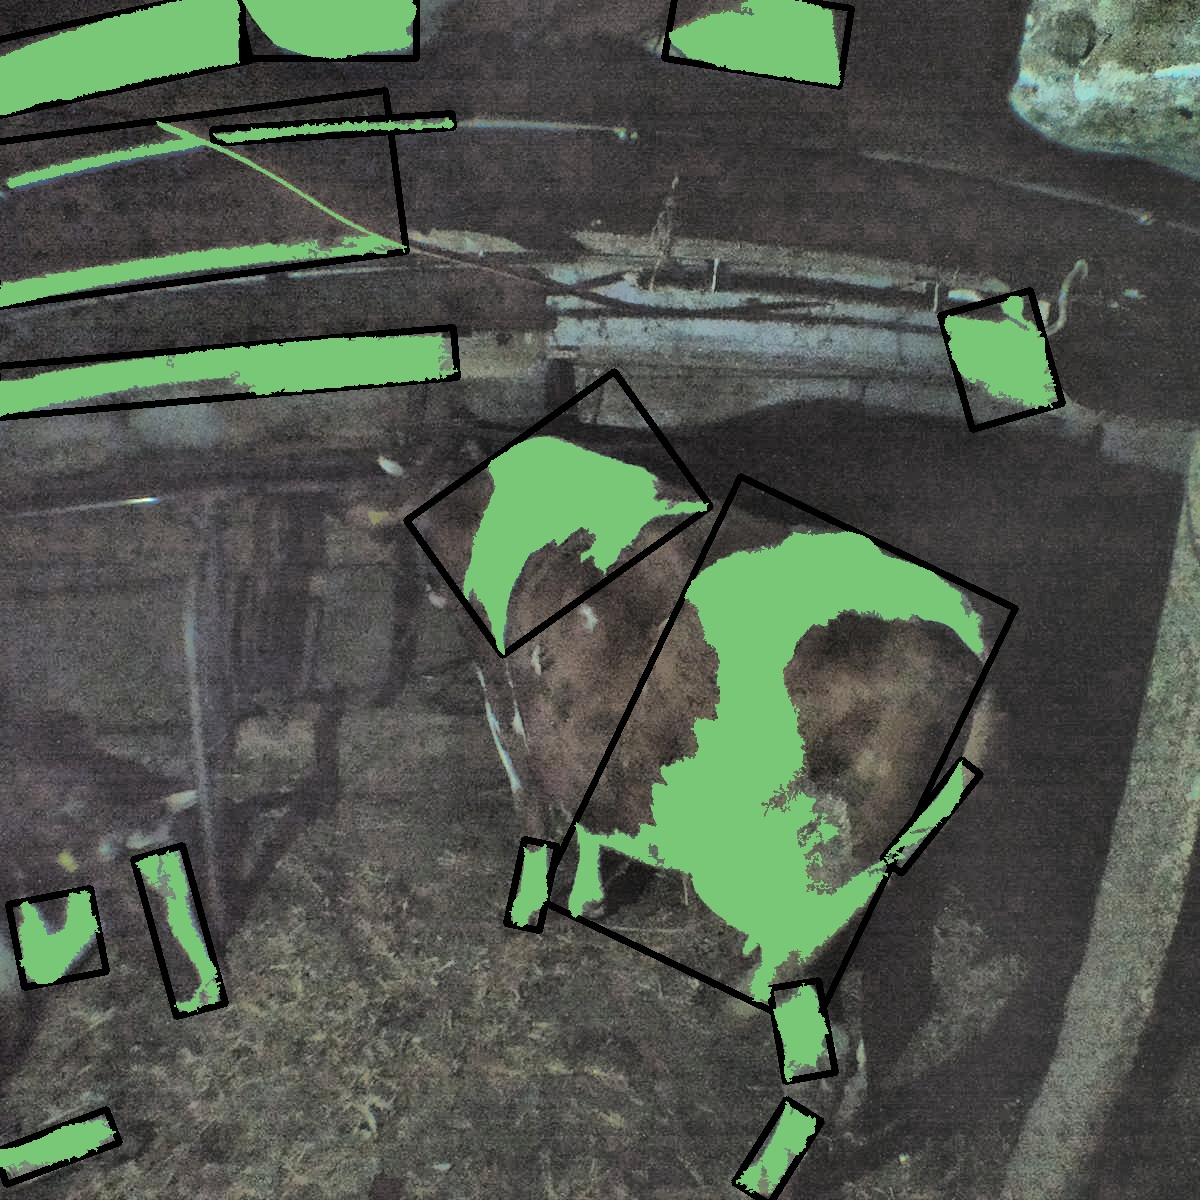
\includegraphics[scale=0.3]{Grafiken/resultate/resultatStanding2.jpg}
	\caption{Korrektes Ergebnis von Analyse der stehenden Kuh} 
	\label{fig: Korrektes Ergebnis von Analyse der stehenden Kuh} 
\end{figure}



\begin{figure}[H]
	\center
	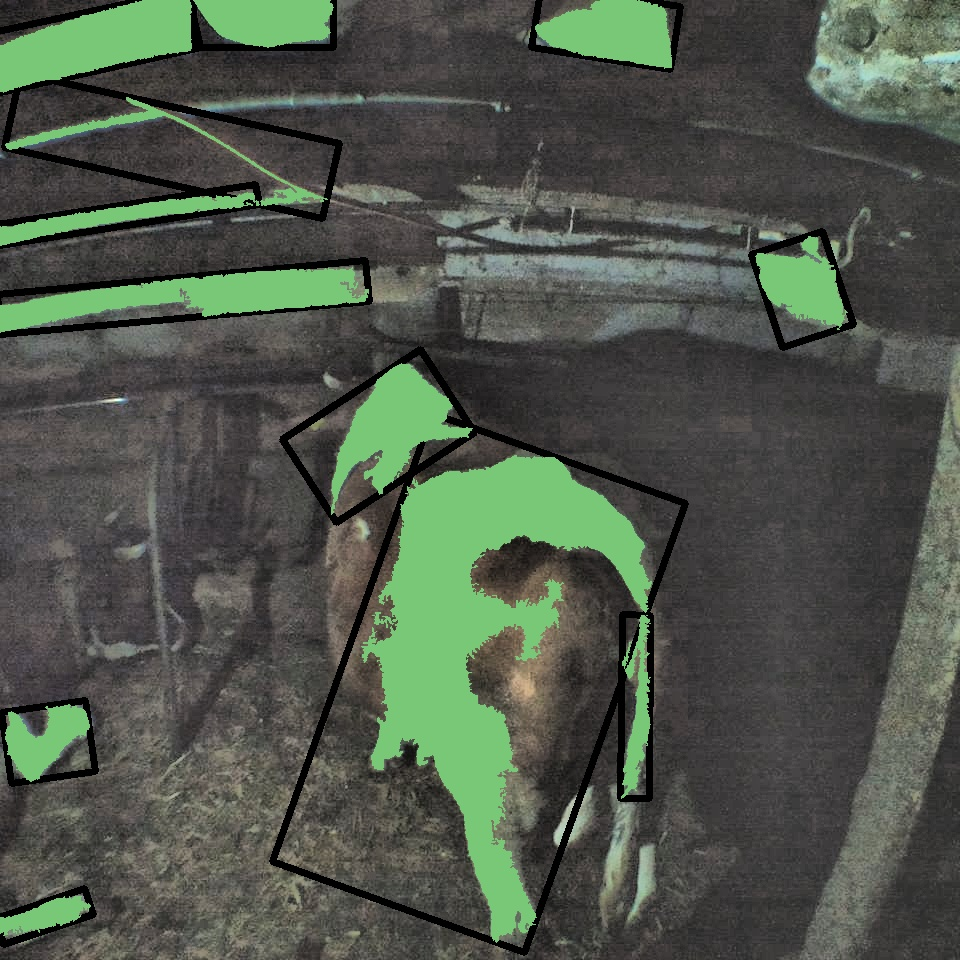
\includegraphics[scale=0.3]{Grafiken/resultate/resultatStanding1.jpg}
	\caption{Weiteres korrektes Ergebnis von Analyse der stehenden Kuh} 
	\label{fig: Weiteres korrektes Ergebnis von Analyse der stehenden Kuh} 
\end{figure}

In den Abbildungen \ref{fig: Korrektes Ergebnis von Analyse der Kuh in Seitenlage} und \ref{fig: Weiteres korrektes Ergebnis von Analyse der Kuh in Seitenlage} erkennt das System korrekterweise, dass sich die abgebildete Kuh in Seitenlage befindet. 

\begin{figure}[H]
	\center
	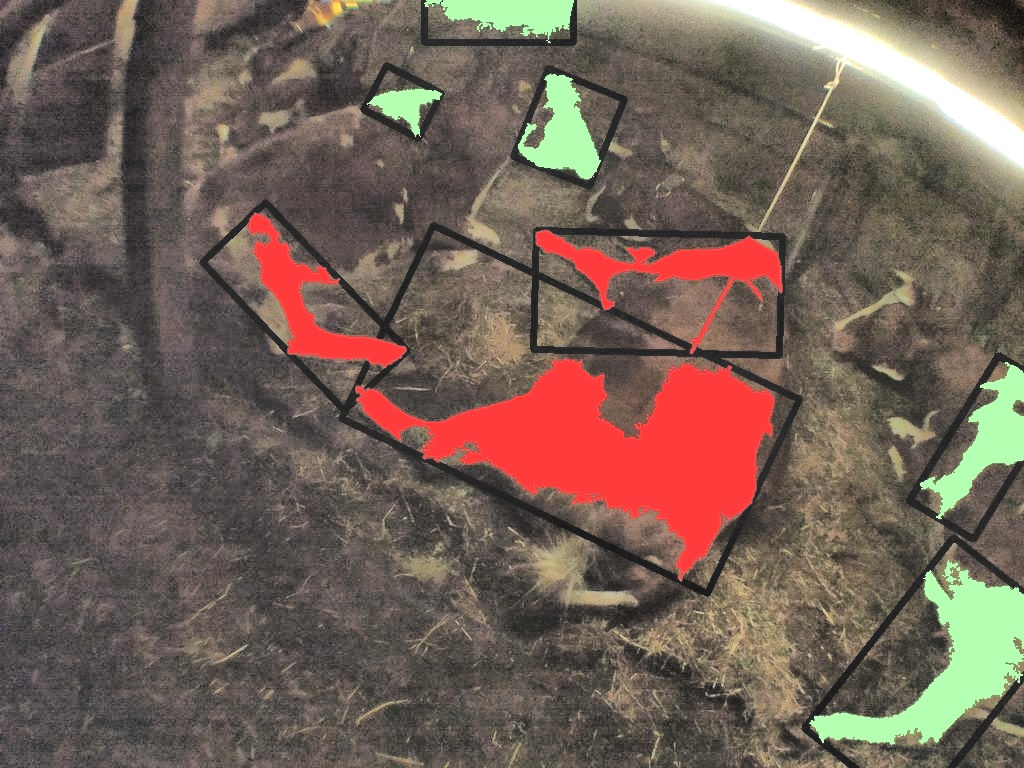
\includegraphics[scale=0.43]{Grafiken/resultate/resultatLying1.jpg}
	\caption{Korrektes Ergebnis von Analyse der Kuh in Seitenlage} 
	\label{fig: Korrektes Ergebnis von Analyse der Kuh in Seitenlage} 
\end{figure}


\begin{figure}[H]
	\center
	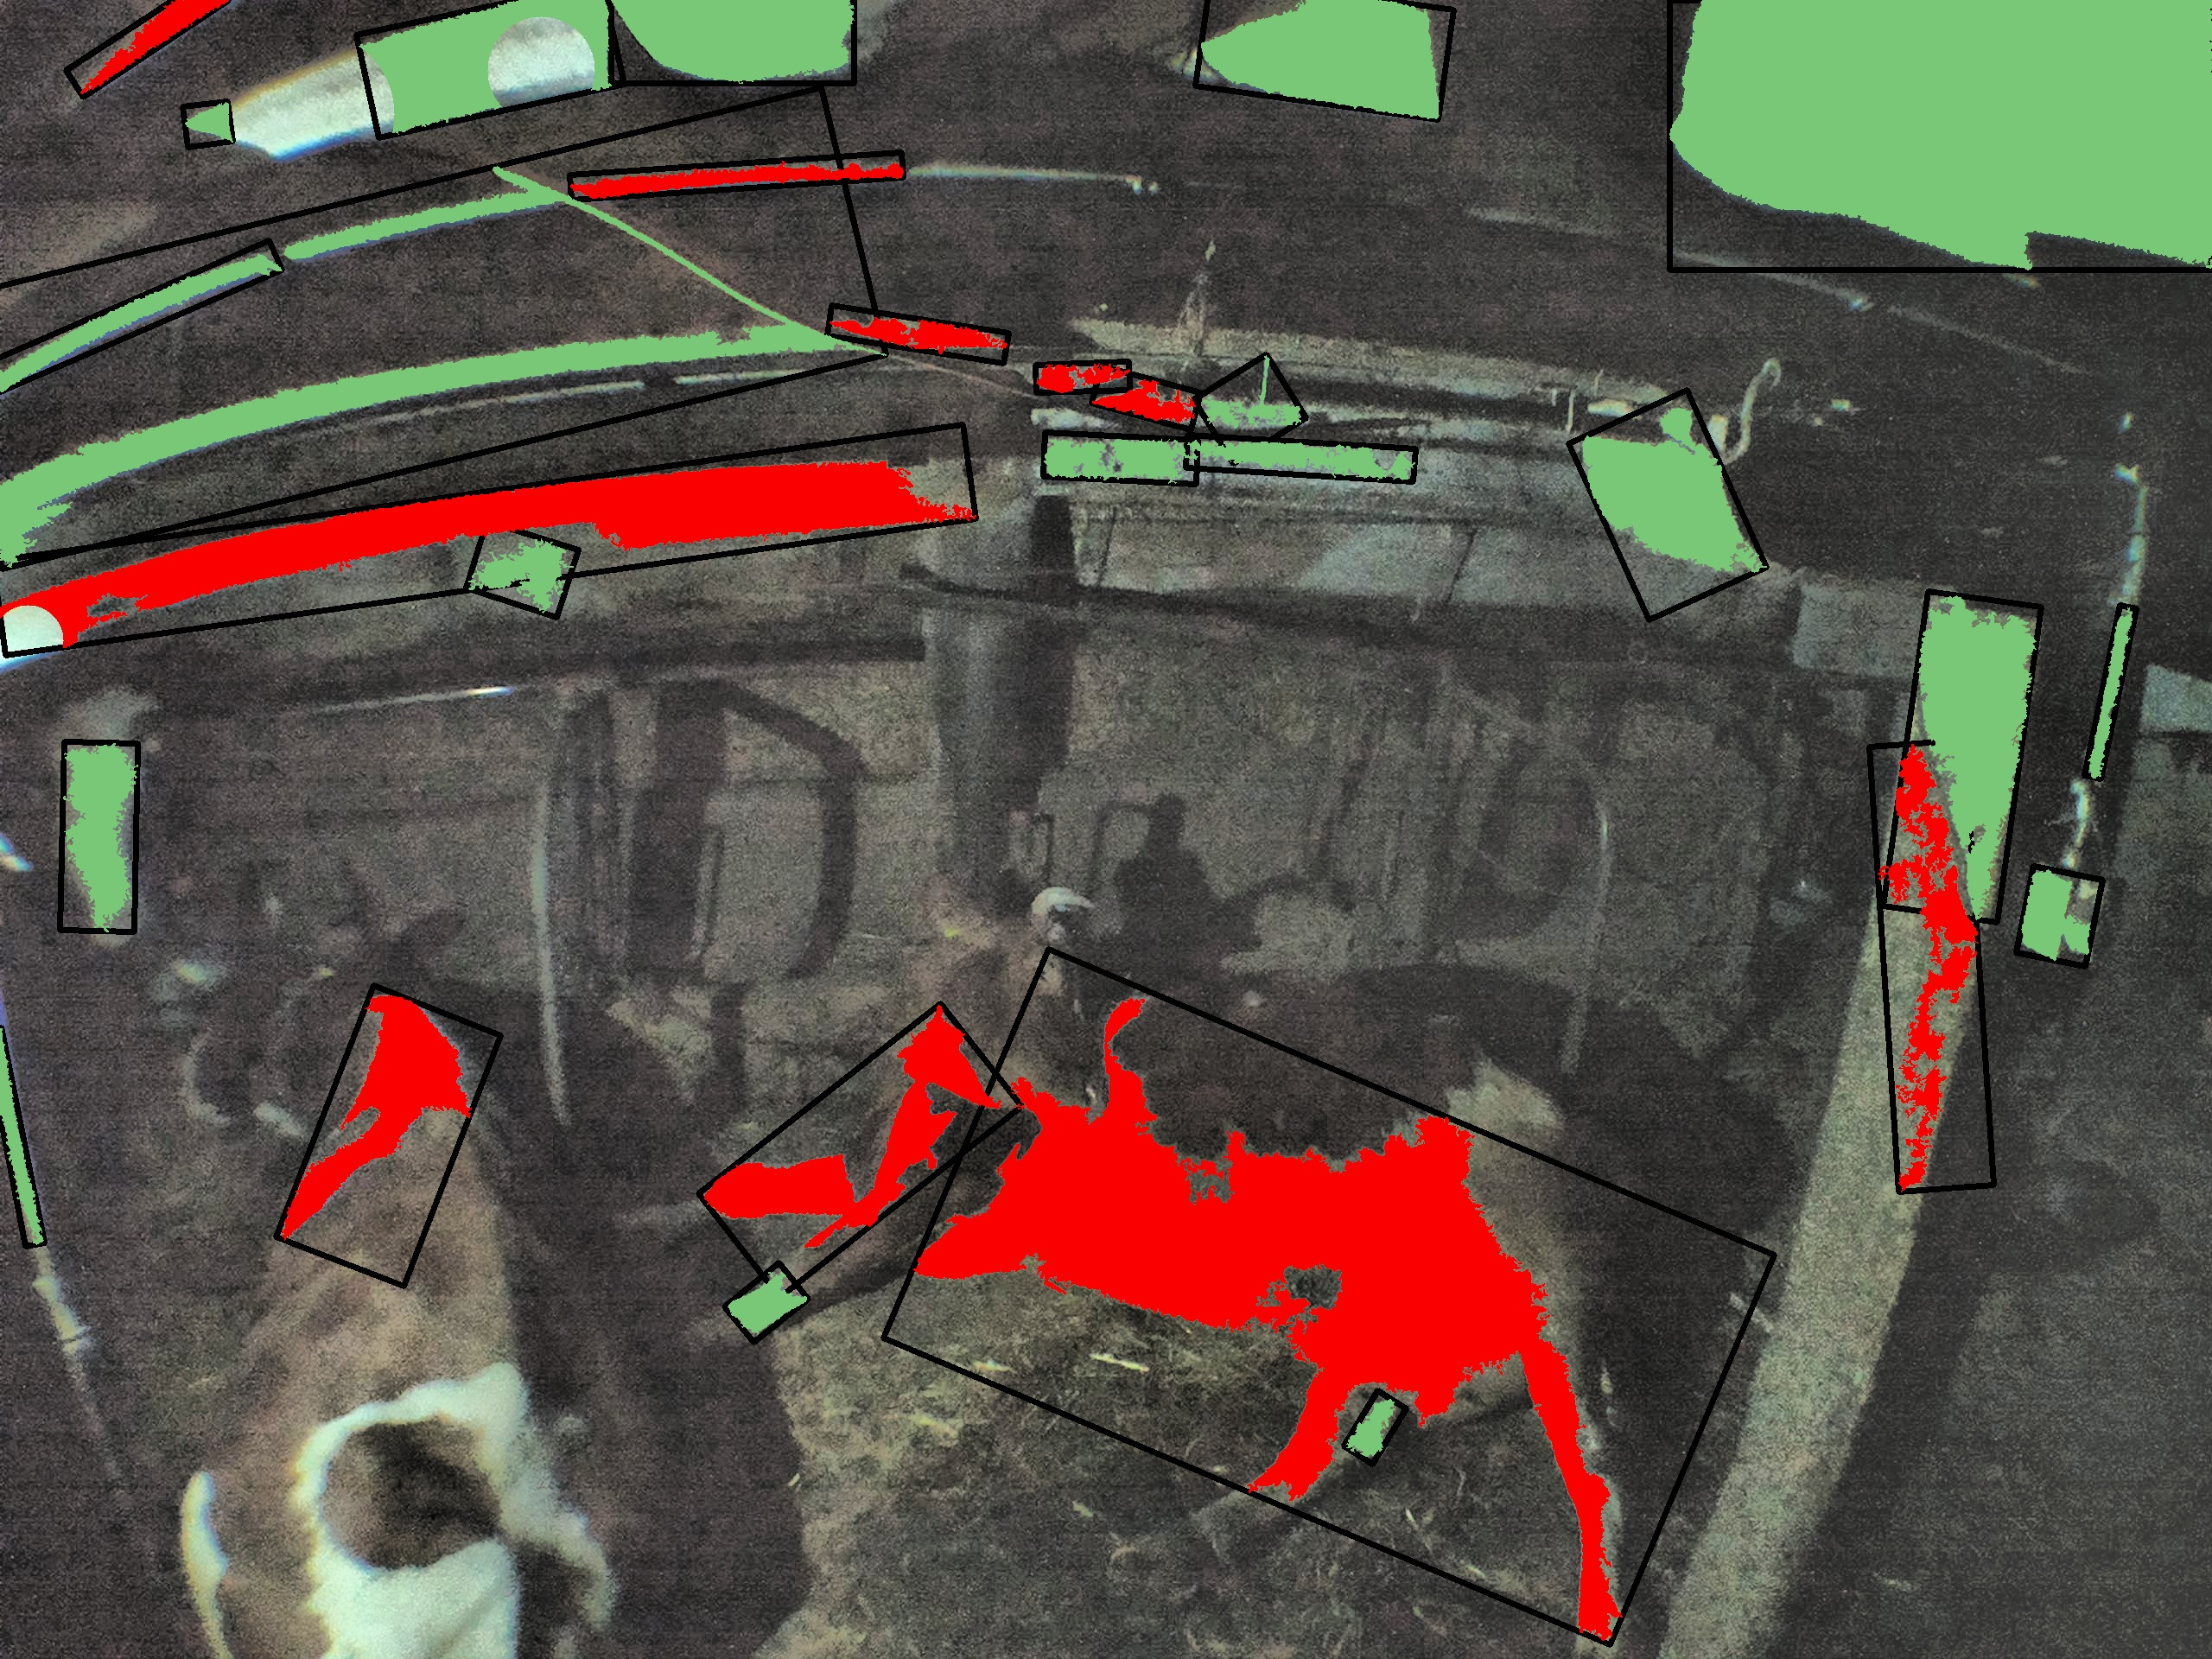
\includegraphics[scale=1.5]{Grafiken/resultate/resultatLying2.jpg}
	\caption{Weiteres korrektes Ergebnis von Analyse der Kuh in Seitenlage} 
	\label{fig: Weiteres korrektes Ergebnis von Analyse der Kuh in Seitenlage} 
\end{figure}

Um die bestmöglichen Ergebnisse zu erzielen, ist jedoch jeweils eine angepasste Konfiguration notwendig.
Einerseits muss jeweils eingestellt werden, ob nur die Farbwerte der Lampe als unwichtige Farbewerte zu interpretieren sind oder noch weitere Farben einen unwichtigen Bereich darstellen. Um zusätzliche Farbwerte als unwichtig zu deklarieren, kann diese Option mittels \texttt{ADVANCED_UNIMPORTANT_COLOR_RANGE=True} aktiviert werden. Anschliessend können beliebig viele Farbbereiche der Liste \texttt{additionalUnimportantColorRanges} hinzugefügt werden. Das System verarbeitet diese Liste an Farbbereichen und maximiert die als unwichtig identifizierbaren Bereiche.

Andererseits muss eingestellt werden, ob die Konturen nach Winkel gefiltert werden. Das System filtert die Konturen standardmässig nach Winkel, ermöglicht aber eine Deaktivierung dieser Funktionalität mittels \texttt{FILTER_BY_ANGLE=False}. Die fachliche Begründung dafür ist, dass nicht immer alle Boxen im Stall besetzt sind. Wenn eine Kuh neben einer leeren Box kalbert, kann sie sich quer über zwei Boxen legen zum Kalbern. In dieser Situation ist eine Filterung der Konturen nach Winkel fachlich nicht sinnvoll.

Das System bietet zahlreiche weitere Konfigurationsmöglichkeiten. Die zwei genannten Optionen bilden fachlich  erheblichen Mehrwert. Experten können ohne Wissen über die technische Implementierung das System so konfigurieren, dass die Ergebnisse weiter verbessert werden. 

Als Beispiel dient das Ergebnis, welches in Abbildung \ref{fig: Weiteres Ergebnis von Kuh in Seitenlage} sichtbar ist. Dieses Resultat wurde mit \texttt{FILTER_BY_ANGLE=False} und und \texttt{ADVANCED_UNIMPORTANT_COLOR_RANGE = False} erzielt. 
\begin{figure}[H]
	\center
	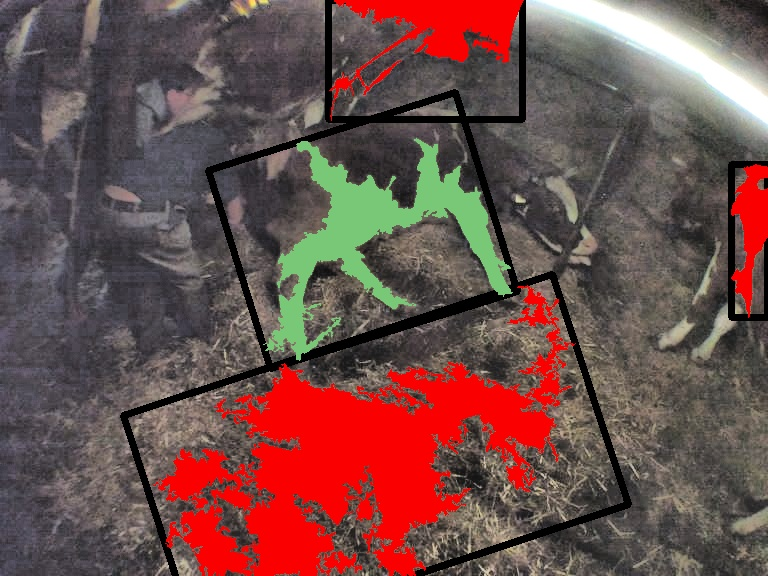
\includegraphics[scale=0.5]{Grafiken/resultate/resultatFehlerhaft.jpg}
	\caption{Fehlerhaftes Ergebnis von Analyse der Kuh in Seitenlage} 
	\label{fig: Fehlerhaftes Ergebnis von Analyse der Kuh in Seitenlage} 
\end{figure}

Durch die Konfiguration von \texttt{ADVANCED_UNIMPORTANT_COLOR_RANGE=True} und der Ergänzung zur Detektierung von unwichtigen Farbwerten im Bereich des Strohs und sehr hellen Bereichen im oberen Bildbereich kann das Ergebnis verbessert werden. In Abbildung \ref{fig: Verbessertes Ergebnis von Analyse der Kuh in Seitenlage} wird das Stroh nicht mehr fälschlicherweise als Kontur der Kuh interpretiert. Das Gesamtergebnis der Analyse ist trotzdem falsch, die Seitenlage wird nicht erkannt, weil der das umschliessende Rechteck den Schwellwert für die minimale Aspect Ratio nicht erreicht. Dennoch veranschaulicht dieses Beispiel den erheblichen Mehrwert des konfigurierbaren Systems.

\begin{figure}[H]
	\center
	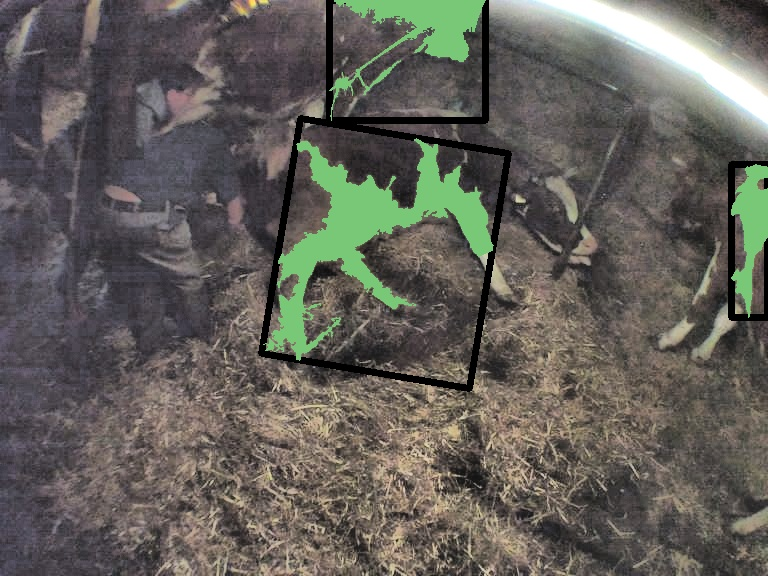
\includegraphics[scale=0.5]{Grafiken/resultate/verbessertesResultat.jpg}
	\caption{Verbessertes Ergebnis von Analyse der Kuh in Seitenlage} 
	\label{fig: Verbessertes Ergebnis von Analyse der Kuh in Seitenlage} 
\end{figure}


Die im Rahmen der Bachelor-Arbeit erarbeiteten Lieferergebnisse werden per E-Mail an Prof. Dr. Patrizio Collovà und Dr. Klaus-Georg Deck geschickt. Dies umfasst nebst dem Bericht ein Archiv mit dem Quellcode des entwickelten Systems, den erstellen Modellen und dem Code zur Analyse der Daten aus den Interviews. 

Zudem ist der gesamte Quellcode des entwickelten Systems auf GitHub verfügbar\footnote{\url{https://github.com/dominiquemueller/birth-detector}}. 